% SO(3) rotation diagram for notebook 01: a frame rotated by angle theta about
% the z-axis (out of the page). Exponential coordinates omega_hat * theta.
% Standalone: compiles with `lualatex rotation_so3.tex`; loaded via render_tikz_file.
\documentclass[tikz,border=4pt]{standalone}
\usepackage{amsmath}
\usepackage{tikz}
\usetikzlibrary{arrows.meta,calc,angles,quotes}
\begin{document}
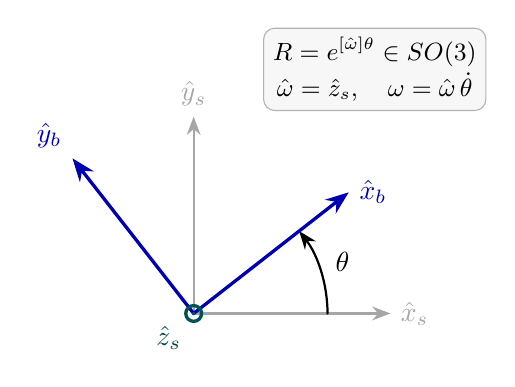
\begin{tikzpicture}[>=Stealth,scale=2.0,line cap=round,line join=round]
  \def\th{38}  % rotation angle (degrees) for drawing

  % --- fixed frame {s} (gray) ---
  \draw[->,gray!70,thick] (0,0) -- (1.25,0) node[right]{$\hat{x}_s$};
  \draw[->,gray!70,thick] (0,0) -- (0,1.25) node[above]{$\hat{y}_s$};

  % --- rotated body frame {b} = R(theta) {s} (colored) ---
  \draw[->,blue!70!black,very thick] (0,0) -- (\th:1.25) node[right]{$\hat{x}_b$};
  \draw[->,blue!70!black,very thick] (0,0) -- ({\th+90}:1.25) node[above left]{$\hat{y}_b$};

  % --- rotation axis z_s out of the page (omega) ---
  \draw[teal!65!black,very thick] (0,0) circle (0.05);
  \fill[teal!65!black] (0,0) circle (0.012);
  \node[teal!55!black,below left=1pt] at (0,0) {$\hat{z}_s$};

  % --- angle theta between x_s and x_b ---
  \draw[->,thick] (0.85,0) arc (0:\th:0.85);
  \node at ({\th/2}:1.0) {$\theta$};

  % --- exponential-coordinate label ---
  \node[align=center,draw=black!30,rounded corners,fill=black!3,font=\small]
        at (1.15,1.55)
    {$R=e^{[\hat{\omega}]\theta}\in SO(3)$\\[2pt]
     $\hat{\omega}=\hat{z}_s,\quad \omega=\hat{\omega}\,\dot{\theta}$};
\end{tikzpicture}
\end{document}
